%!TEX root = thesis.tex
\chapter{Demonstrator}
\label{chap:demonstrator}

To demonstrate the work described in the previous chapters in a real world
application, a ball on plate system is presented in the following sections.
The demonstrator tries to balance a ball by tracking its position and
adjusting the angle of the underlying plate, thus allowing to compensate
external impacts and keeping the ball in the center. Therefore, the plate
itself is mounted on top of a Stewart platform and has a resistive touchscreen
attached to it. While the Stewart platform offers the ability to rotate the
plate around arbitrary axes, the touchscreen provides precise and low latency
positioning information of the ball.

The control of the platform is implemented by a \ac{PAC} based on the previous
considerations, including analog I/O, low latency data paths and control
loops, as well as self-adaptive capabilities. The different components of the
system are described in detail in the following sections. These include the
kinematics of the Stewart platform, the touchscreen interface and control
algorithms for balancing the ball.

\section{Stewart Platform}
The Stewart platform was introduced by D. Stewart in 1965 \citep{Ste65} and
gained popular resarch interest in robotics \citep{Szu13}, concerning
kinematics, dynamics or work space estimations. However, outside the
scientific community the Stewart platform was not widely adopted and most
designs are constrained to applications requiring \ac{6DoF}, for instance
flight simulators or \ac{CNC} machining centers. Although a Stewart platform
provides many potential advantages, sophisticated synthesis and simulation
tools are missing \citep{Ji96}. Against the background of increasing
computational capabilities and more efficient \ac{CAD} tools, this situation
might change in the future. In the scope of this thesis, the Stewart platform
promises to be a sophisticated development platform, involving computationally
expensive calculations for its kinematics and the need for additional I/O
capabilities.

The following sections introduce the architecture of the Stewart platform in
general and the variant used in this thesis, specify the used notations and
solve the inverse kinematics problem.

\subsection{Architecture}
While Stewart introduced the general idea of a Stewart platform in his work in
1965 \citep{Ste65}, a strict definition is missing in the literature. The only
commonality is the characterization as a parallel manipulator \citep{Szu13},
consisting out of a bottom base and an upper platform. Compared to a serial
manipulator, it consists out of multiple serial chains controlled
simultaneously and connected to a single end-effector. While this design
provides unique benefits like high accuracy, better load-to-weight ratios and
improved rigidity, it limits the available work space and causes highly
nonlinear behavior.

%\begin{figure}
%	\centering
%	\begin{subfigure}{0.3\textwidth}
%		\centering
%		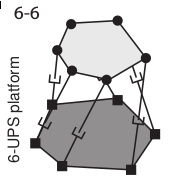
\includegraphics[width=\textwidth]{../figures/stewart_architectures_c}
%		\caption{6-UPS}
%		\label{fig:stewart_architectures_a}
%	\end{subfigure}
%	\begin{subfigure}{0.3\textwidth}
%		\centering
%		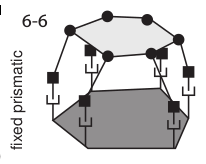
\includegraphics[width=\textwidth]{../figures/stewart_architectures_d}
%		\caption{Fixed prismatic}
%		\label{fig:stewart_architectures_b}
%	\end{subfigure}
%	\begin{subfigure}{0.3\textwidth}
%		\centering
%		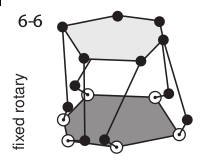
\includegraphics[width=\textwidth]{../figures/stewart_architectures_e}
%		\caption{Fixed rotary}
%		\label{fig:stewart_architectures_c}
%	\end{subfigure}
%	\caption{Different variants of Stewart platforms \citep[adopted from][]{Szu13}}
%	\label{fig:stewart_architectures}
%\end{figure}
The different variant of a Stewart platform vary in the type of the
connections and actuators, as well as their spacial configuration, i.e. the
positioning of the different connections. The most common realization utilizes
six prismatic actuator, for example hydraulic pistons or linear motors. It is
often referred to as Hexapod and associated with the term Stewart platform,
not least because of its similarity to the original design proposed by
Stewart. Other architectures utilize fixed prismatic or rotary actuators to
vary the lengths of the six legs. All of these variants have its unique
benefits and drawbacks. Since the actuators in the latter design can be
realized as commonly available servo motors, it gained popularity, especially
for low-cost designs and first prototypes. Therefore, this thesis focuses on a
servo-based architecture as shown in figure
\ref{fig:stewart}. The mechanical design and construction was not done in this
thesis, but adopted from a previous work.
\begin{figure}
	\centering
	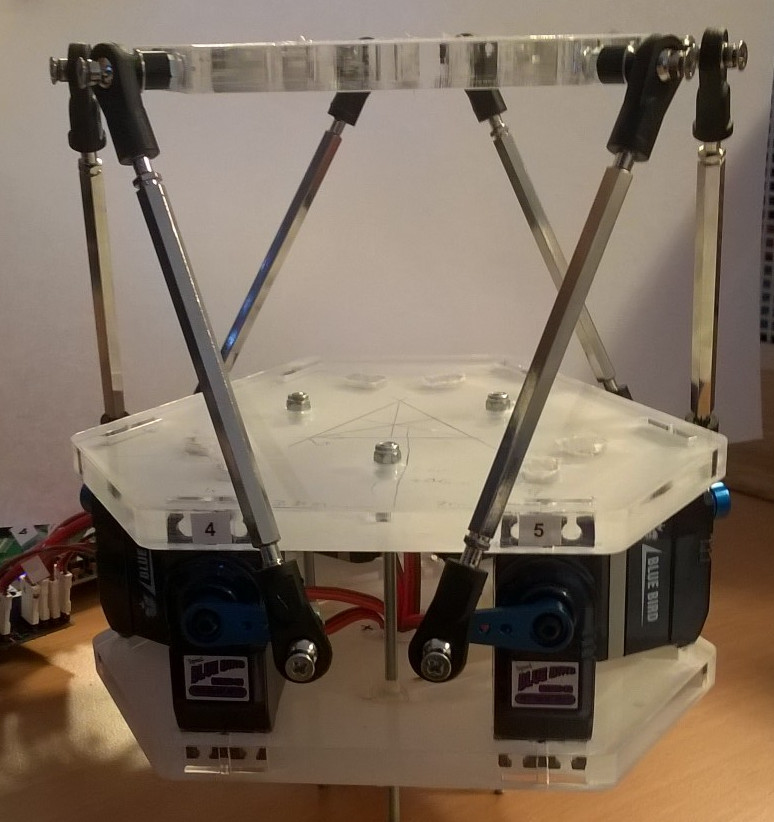
\includegraphics[width=6cm]{../figures/stewart}
	\caption{Construction of the Stewart platform prototype}
	\label{fig:stewart}
\end{figure}

\subsection{Construction and Notation}
This section introduces the basic notations, coordinate systems and dimensions
of the Steward platform used in this thesis. Consider figure
\ref{fig:stewart_notation}, showing different views annotated with the
relevant notations.
\begin{figure}
	\centering
	\begin{subfigure}{0.49\textwidth}
		\centering
		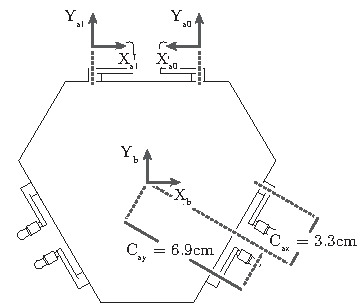
\includegraphics{../figures/stewart_base}
		\caption{Top view of base}
		\label{fig:stewart_base}
	\end{subfigure}
	\begin{subfigure}{0.49\textwidth}
		\centering
		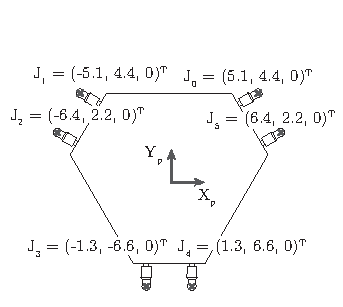
\includegraphics{../figures/stewart_platform}
		\caption{Top view of platform}
		\label{fig:stewart_platform}
	\end{subfigure}
	\par\bigskip
	\begin{subfigure}{0.49\textwidth}
		\centering
		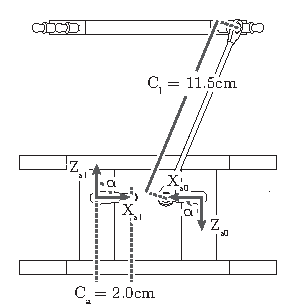
\includegraphics{../figures/stewart_side}
		\caption{Side view}
		\label{fig:stewart_side}
	\end{subfigure}
	\caption{Notations for the Stewart platform}
	\label{fig:stewart_notation}
\end{figure}

As already described previously, the system consists out of a lower base and
an upper platform, connected by six legs. For both, the base and platform, a
particular coordinate system is introduced as shown in figures
\ref{fig:stewart_base} and \ref{fig:stewart_platform}. While the origin of the
base coordinate system $B$ is located in the center of the base and at the
same height as the shaft of the servos, the origin of platform's coordinate
system $P$ is located exactly at the height of the platform joints
$J_i$. With regard to the platform's coordinate system, the coordinates of the
six joints are annotated in figure \ref{fig:stewart_platform}.

Additionally, each servo specifies its own coordinate system $S_i$, located at
the intersection point of the servo's shaft and the servo's joint position.
Thereby, the y axis points away from the base and the x axis along the servo's
arm in neutral position. Resulting from these two axes, the z axis points up
or down, depending of the servo, i.e. for even servos it points down and for
odd servos it point up. Figure \ref{fig:stewart_side} illustrates the servo
coordinate systems and shows the angle $\alpha$ of the servo arm. The
different coordinate systems for even and odd servos allow to handle all
servos analogously and to respect the physical configuration of the servo
arms.

Calculating the inverse kinematics of the platform requires to transform the
joints of the platform to the corresponding servo coordinate system. This is
done in two steps, by transforming them to $B$, and finally to $S_i$. While
the transformation to the base coordinate system $B$ is trivial, by simply
adding an offset $C_h$ to the z coordinate, transforming the resulting point
to the servo coordinate system $S_i$ requires more sophisticated calculations,
including rotation and scaling. At first, the base coordinate system is
rotated to match the y axis of the appropriate servo coordinate system,
followed by mirroring the x and z axis to fit the desired orientations.
Finally, the origin is translated to match the servo positions by adding and
subtracting $C_{sx}$ and $C_{sy}$ to the x and y coordinates, respectively.

\subsection{Inverse Kinematics}
Taking the basic notations of the previous section as a basis, the inverse
kinematic calculates the required servo angles for a desired angle of the
platform. Unlike for serial manipulators, the inverse kinematics of a Stewart
platform has a unique analytic solution, while the forward kinematics problem
is highly nonlinear and requires iterative approaches. However, the low-cost
variant utilizing rotary instead of linear actuators introduces additional
calculations to calculate the required servo angles from the desired leg
lengths.

Assuming, that the desired angle of the platform is given by a rotation axis
$r$ and a rotation angle $r_a$, equation \ref{eq:platform_rot} shows the
calculation of the required platform joint's positions.
\begin{equation}
J'_i = 
\begin{pmatrix}
\left[\left(1 - \cos(r_a)\right) r_x r_x + \cos(r_a)\right] J_ix + \left[\left(1 - \cos(r_a)\right) r_x r_y\right] J_iy\\
\left[\left(1 - \cos(r_a)\right) r_x r_y\right] J_ix + \left[\left(1 - \cos(r_a)\right) r_y r_y + \cos(r_a)\right] J_iy\\
\left[-r_y \sin(r_a)\right] J_ix + \left[r_x \sin(r_a)\right] J_iy\\
\end{pmatrix}
\label{eq:platform_rot}
\end{equation}
Transforming these position to the appropriate servo coordinate systems as
described in the previous section allows to calculate the distance between the
servo joint and the platform joint. While for a linear actuator this would be
the solution, rotary actuators can not vary the length of the legs directly.
Therefore, the angle $\alpha$ must be adjusted in a way, that the distance
between its joint and the platform joint is equal to the fixed leg length
$C_l$. While there exist an analytic solution for this problem, it includes
terms of higher degree and complex operations like $\arctan$ and square roots.
Therefore, an iterative approach was chosen to find the appropriate angle.
More details on the concrete implementation of this iterative approach will be
covered in the implementation section.

\section{Touchscreen}
To track the ball's position on the plate, a resistive touchscreen is mounted
on top of the plate and touched by the ball. Compared to, for example camera
based tracking techniques, a touchscreen provides low latency data,
independent from external influences like lighting conditions or camera
movements. Furthermore, it requires less computational effort, as well as a
more compact setup.

The following subsections introduce briefly the fundamental principles of the
resistive touchscreen technology and covers the use in the prototype.

\subsection{Resistive Touchscreen Technology}
An analog resistive touchscreen consists out a glass substrate and a flexible
film, both coated with a conductor \ac{ITO} \citep{Wal12}, as shown in figure
\ref{fig:touch_build}.
\begin{figure}
	\centering
	\begin{subfigure}{0.49\textwidth}
		\centering
		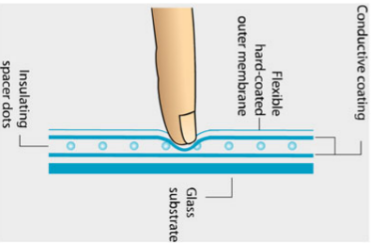
\includegraphics{../figures/touch_build}
		\caption{Construction of resistive touchscreen}
		\label{fig:touch_build}
	\end{subfigure}
	\begin{subfigure}{0.49\textwidth}
		\centering
		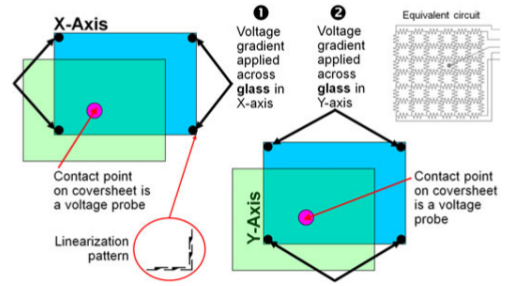
\includegraphics{../figures/touch_five}
		\caption{Five-wire touchscreen}
		\label{fig:touch_five}
	\end{subfigure}
	\caption{Analog resistive touchscreen technology \citep[adapted from][]{Wal12}}
	\label{fig:touch}
\end{figure}
The two conductive surfaces are facing each other and
are separated by insulating spacer dots \citep{Wal12}. When a voltage is
applied across the surfaces and the flexible film is pressed down, the two
surfaces make electrical contact, resulting in a voltage divider created by
the resistance of the \ac{ITO}. Measuring the ratio of the different voltages
allows to calculate the touch position.

Basically, there exist three major variants of resistive touchscreens, namely
four-wire, five-wire and eight-wire touchscreens, differing in the number of
connections to the sensor \citep{Wal12}. For the demonstrator, a five-wire
touchscreen was used as shown in figure \ref{fig:touch_five}, due to its
increased durability and sustainability. The X and Y voltages are applied to
the four corners of the lower glass, while the upper film is used only as a
contact point to measure the voltage at the touch position (wiper). To
determine, for example, the X position, a voltage is applied to the two left
corners, while two right corners are connected to ground.

\subsection{Interfacing the Touchscreen}
To interface the touchscreen, voltage needs to be applied to different corners
of the touchscreen, while all other ones needs to be connected to ground.
Therefore, regular digital I/O are sufficient, setting their output to 1 or 0,
respectively. To measure the voltage at the touch point through the viper, an
\ac{ADC} with suitable input ranges is required. To eliminate noise caused by
an unstable voltage source, the \ac{ADC} should be connected in a differential
fashion to the wiper and the supply voltage. This improves the reliability and
minimizes the effects of voltage fluctuations \citep{OOD00}.

In this work, the pre-assembled evaluation module ADS7845EVM \citep{ADS06} was
used. While the ZedBoard provides both digital I/O and an on-chip \ac{ADC}
which could be utilized to interface a touchscreen, additional circuits would
be required to meet the \ac{ADC}'s input requirements. Since circuit design is
not target of this thesis, a pre-assembled evaluation module was chosen. It
provides an appropriate connector for the touchscreen and interfaces with the
\ac{FPGA} via the \ac{SPI} interface as shown in figure \ref{fig:touch_spi}.
\begin{figure}
	\centering
	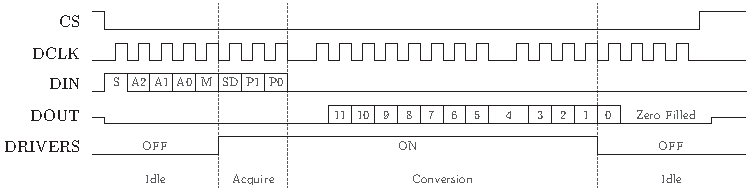
\includegraphics{../figures/touch_spi}
	\caption{\acs{SPI} interface of the ADS7845 touch controller \citep[adapted from][]{ADST06}}
	\label{fig:touch_spi}
\end{figure}
A single conversion is done in 24 clock cycles with a period of
$\SI{400}{\nano\second}$ by sending eight configuration bits to the controller
and receiving the converted voltage at the touch position as a 12 bit integer.
The configuration bits sent in the first byte include the channel selection
\emph{A2} - \emph{A0}, i.e. the x and y directions, mode selections and power
down options. The \emph{SD} bit selects between single-ended and differential
mode, \emph{M} selects between eight and twelve bit conversion and \emph{P1} -
\emph{P0} control the power down between conversions. After the control byte
is sent, the controller enters the conversion mode and performs the analog-to-
digital conversion in the next twelve clock cycles. In the 13th clock cycle
the last bit is transferred, followed by three zero bits to complete the last
byte. Therefore, 48 clock cycles are necessary to read the x and y coordinate
of the touch position, i.e. around $\SI{20}{\micro\second}$. Note, that these
information only imply a single measurement, while, as stated later, for a
precise positioning information multiple conversions are required.

To connect the controller evaluation module to the ZedBoard, regular digital
I/Os are required for the serial interface, as well as a $\SI{3.3}{\volt}$
voltage supply, provided by one of the \ac{Pmod} connectors.

\section{\acs{PID} Control}
Tracking of the ball's position and adjusting the plate's angle appropriately,
allows to stabilize the ball at a desired position, for example at the center.
This task is a typical control application and should be implemented by the
well-known \ac{PID} controller, consisting out of a proportional, integral and
derivative term. \ac{PID} controllers are widely adopted in the field of
industrial control and have a long history of use, surviving several changes
of technology \citep{Joh05}. Even complex applications comprise control
networks out of basic \ac{PID} loops.

Figure \ref{fig:pid_rep} \todo{fix wrong PD in controller figure} illustrates the concept of a \ac{PID} controller with
regard to the ball-on-plate application as the process of the control loop.
\begin{figure}
	\centering
	\centering
	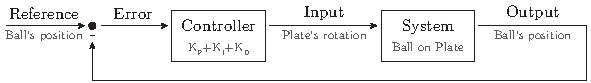
\includegraphics{../figures/pid_rep}
	\caption{Representation of controlled system}
	\label{fig:pid_rep}
\end{figure}
The platform's rotation constitutes the manipulated variable, while the ball's
position represents the controlled variable. The error vector is calculated as
the difference of the target position and the current position, i.e., since
the target position is the center of the plate, the negated position of the
ball. Vividly, the resulting controller output represents the acceleration
required to push the ball in the desired direction. To achive this
acceleration, the platform needs to bo rotated around an axis perpendicular to
the acceleration vector and by an angle, proportional to the length of the
vector. These two values can be determined by applying geometric calculations
and fed into the inverse kinematics algorithm to achieve the correct rotation.
Note, that the controller output vector does generally not point to the target
position, since the derivative term compensates the velocity of the ball.

While the implementation of a \ac{PID} controller is well-known, the
challenging part is to tune its parameters, i.e. the factors for the
proportional, integrative and derivative terms. Typically, simulations are
used to represent the controlled process by a mathematical model and
numerically calculating optimal parameters. However, the focus of this thesis
does not lay on controller design and, therefore, appropriate values where
determined by systematic experiments.

\section{Implementation}
While the previous sections covered the fundamentals for the demonstrator and
addressed the main problem definitions, this section focuses on the
implementation of the different components. Consider figure
\ref{fig:demo_structure}, illustrating the overall structure of the system.
\begin{figure}
	\centering
	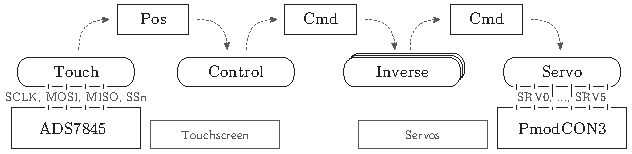
\includegraphics{../figures/demo_structure}
	\caption{Overall structure of the demonstrator}
	\label{fig:demo_structure}
\end{figure}
It consists out of four types of ReconOS threads, which are representing the
control loop of the ball on plate application and are synchronized via
mailboxes to each other. The \emph{Touch} thread interfaces with the external
ADS7845 touch controller by implementing an \ac{SPI} master and provides the
positioning information to the \emph{Control} thread. That implements the
\ac{PID} controller and passes the manipulated variable, i.e. the rotation of
the platform, to the \emph{Inverse} thread. Since the inverse kinematic
constitutes the most computational intensive task and must be performed for
each of the six legs, it is parallelized in multiple threads, each one
calculating a single servo position. Therefore, one to six
\emph{Inverse} threads might be instantiated.

While the \emph{Touch} and \emph{Servo} threads must be implemented as
hardware threads, allowing them to interface with the I/O ports of the FPGA,
the remaining partitioning can be performed arbitrarily. Both the control and
inverse kinematics implementations are available for hardware synthesis, as
well as for software compilation.

\paragraph{Touch} As described in the previous section on the touchscreen
technology, an ADS7845EVM evaluation module is utilized in this work. The
\emph{Touch} thread implements the \ac{SPI} master according the ADS7845's
specifications and provides positioning information to the other threads. The
\ac{SPI} controller generates the required $\SI{2.5}{\mega\hertz}$ clock and
implements shift registers for both sending and receiving data. While the
touch controller returns a 12 bit value representing the measured voltage at
the sensing position, the touch thread converts them into coordinates
representing the ball's position in the plate's coordinate system by applying
translations and scaling. Additionally, to reduce noise in the ball's
position, multiple measurements are performed in a single scan cycle. Thereby,
a series of measurements is discarded, when a pair of consecutive readouts
differs noticeably, for example because of insufficient pressure applied to
the touchscreen. Only if the measurements passes the validity check, their
average is used for calculating the ball's position. Since this procedure
results in a varying acquisition time, the touch thread also monitors the
actual period of time past the last measurement and reports it to the control
thread.

\paragraph{Control} The \emph{Control} thread implements the \ac{PID}
controller as described in the previous section. Therefore, it receives the
ball position from the \emph{Touch} thread, calculates the error vector and
applies the \ac{PID}control algorithm as sketched in listing \ref{lst:pid} for
the x coordinate.
\begin{lstlisting}[
	language=VHDL,
	caption={\acs{PID} implementation},
	label={lst:pid},
	float=tb
]
error_x_diff = (error_x - error_x_last) / delta;
error_x_sum += error_x * delta;
ctrl_x_p = KP * error_x;
ctrl_x_i = KI * error_x_sum;
ctrl_x_d = KD * error_x_diff;
ctrl_x = ctrl_x_p + ctrl_x_i + ctrl_x_d;
\end{lstlisting}
The proportional component is directly represented by the current error, while
the derivative and integral components are calculated via the delta variable,
representing the time period since the last value. By multiplying each
component with the \ac{PID} parameters \emph{KP}, \emph{KI} and \emph{KD}, the
resulting control output is determined. Since the inverse kinematics threads
require a rotation axis and an absolute angle to rotate the plate, the output
vector is used to calculate its perpendicular vector of length one as the
rotation axis and its length as the rotation angle.

\paragraph{Inverse} The computationally most demanding component of the
application is the solution of the Stewart platform's inverse kinematics
problem. Therefore, it provides  potential for a speedup by a hardware
implementation. The \emph{Inverse} thread receives an axis encoded as two 10
bit integers and an angle encoded as a 9 bit integer, as well as a 3 bit leg
id. Out of these information, it calculates the desired servo angle for the
specified leg. Since the calculation contains many arithmetic operations
including fixed point calculations, it fits perfectly for an implementation in
Vivado HLS. However, while the tool includes a math library, it is not able to
synthesize sine and cosine functions. Therefore, an array synthesized into
block \ac{RAM} is precalculated and used as a lookup-table. The fixed point
data type \lstinline{ap_fixed<22,10>} is used for all calculations, providing
sufficient accuracy for this application. The returned servo angle is encoded
as an integer of 11 bits, resulting in a precision of $\SI{0.1}{\degree}$. As
already mentioned, the servo angle is calculated out of the leg length by a
linear search over all possible angles. Although an analytical solution could
be formulated, it requires square roots, high potencies and tangent functions,
making it harder to implement on an FPGA.

\paragraph{Servo} The servos of the Stewart platform are controlled by a
\ac{PWM} signal, specifying the angle of the mounted arm. The thread receives
the required angle encoded as an integer together with a servo id via the
incoming mailbox and generates an appropriate \ac{PWM} signal. According the
servo's specification, the pulse must have a width of $\SI{1}{\milli\second}$
to $\SI{2}{\milli\second}$ and a period of $\SI{10}{\milli\second}$ to
$\SI{22}{\milli\second}$, resulting in the minimal or maximal angle,
respectively. Additionally to the control signal, the servos require an
external power supply, since the ZedBoard is not capable of providing
sufficient power. Therefore, the PmodCON3 modules provide a dedicated power
input and connect the control signals directly to the servo.

\section{Self-Awareness}
While the system described so far implements the basic functionality of the
ball-on-plate demonstrator, this section focuses on self-adaption strategies
by extending the demonstrator with a framework to gather self-aware properties
and introducing basic self-expression capabilities to optimize the power
consumption.

As stated in the background chapter, self-aware systems require knowledge of
themselves by acquiring so-called self-*properties, for example by capturing
sensor data or maintaining performance counters. This self-aware knowledge can
then be processed by a self-expression engine to modify the system's behavior
and meet specified requirements. Consider figure \ref{fig:demo_selfaware},
presenting an extended structure of the demonstrator, implementing the concept
of a self-aware system, inspired by \citep{AHL14}.
\begin{figure}
	\centering
	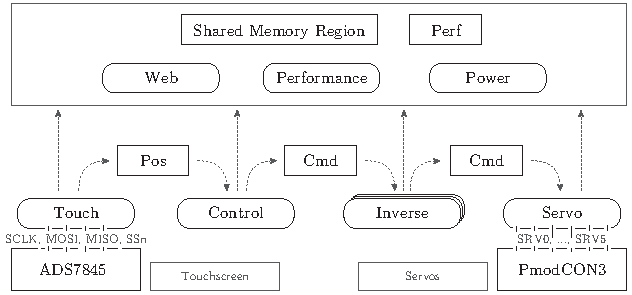
\includegraphics{../figures/demo_selfaware}
	\caption{Extended structure of the demonstrator}
	\label{fig:demo_selfaware}
\end{figure}
A globally accessible shared memory region allows to collect various types of
self-aware properties from different sources. For example, the \emph{Power}
thread acquires sensor data to measure the system's power consumption or the
threads maintain a performance counter. All this data is then utilized by the
\emph{Self} thread, implementing a self-expression engine consisting out of
rules, adjusting parameters of the system. Furthermore, to monitor the
insights of the system, the \emph{Web} threads provides access to several of
the self-properties and parameters via an interactive web interface.

The following subsections explain the different self-properties and how they
are acquired, as well as the adaptions strategies and controlled parameters of
the system.

\subsection{Self-Properties}

The self-properties are acquired by the threads of the system and stored in
the globally accessible shared memory region. While the acquiring of the
properties is typically performed in parallel to the regular processing, the
additional memory access introduces an overhead and might effects the
overall system's performance. However, since the shared memory is not utilized
in the system so far, the overhead can be neglected. For software threads a
single word access is, obviously, not performance critical and a hardware
thread requires less than 10 clock cycles for an access via the memory
subsystem. It does not need to block until the word is written to the system
memory, but can proceed after the request is written to the \ac{MEMIF}
\ac{FIFO}.

To demonstrate self-adaptive capabilities of the system, the power
consumption, the ball's position on the plate and performance measures of the
different threads are acquired and processed by the self-expression engine.

\subsubsection{Power Consumption}
\label{sssec:power}
The power consumption of the system is affected by many components, ranging
from different threads through the entire the Zynq \ac{SoC} to external
devices like the touch controller. Therefore, a fine-grained measurement of
the different component's power consumption would be desirable, allowing a
more sophisticated control.

While more advanced boards include power measurement capabilities through
dedicated components connected to the FPGA, the ZedBoard features a
$\SI{10}{\milli\ohm}$ current sense resistor in series with the
$\SI{12}{\volt}$ input power supply \citep{ZedBoard}. Measuring the voltage
drop at that resistor allows to calculate the current flowing into the board,
and, consequently, the power consumption of the system like in equation
\ref{eq:power}. $V_i$ represents the input voltage from the power supply, i.e.
$\SI{12}{\volt}$, and $V_s$ the measured voltage drop at the shunt resistor.
\begin{equation}
P = V_i I = V_i \frac{V_s}{\SI{10}{\milli\ohm}}
\label{eq:power}
\end{equation}
Since the resistor is placed on the high side, i.e. before any load, it has a
common mode voltage of around $\SI{12}{\volt}$, far exceeding the capabilities
of the on-chip \ac{ADC}. Therefore, the dedicated current sensing amplifier
LTC4151 is used to measure the voltage drop $V_s$. It integrates an
instrumentation amplifier with an appropriate \ac{ADC} and reports data
through the \ac{I2C} interface, connected the Zynq's dedicated \ac{I2C}
controller. This allows to poll the LTC4151 from a regular software thread and
make the measurement data available via the self-properties memory region.
Since this region is globally accessible, both hardware and software threads
can access this data.

Based on the the overall power consumption of the board, different methods for
a more fine-grained measurement can be discussed. Directly measuring the power
consumption of single threads is not feasible, but suitable models could be
applied to estimate the power distribution across the chip. Different works
have dealt with the problem of simulating the power consumption of \acp{FPGA}
\citep{DeTu05,JeCa11} and commercial tools like Xilinx XPower are available to
estimate the resulting drawn. However, the effective switching activity
heavily depends on the input at runtime. Furthermore, external components are
not included in the simulation results and software threads running on an
operating system are heavily dynamic and unpredictable. Especially in case of
self-adaptive systems acquiring parameters at runtime, long running
simulations are not applicable. Therefore, learning strategies observing the
state of the system and its work load seem to be more suitable for power
estimation at runtime. While turning on and off threads or disabling external
components temporarily, the system might be able to learn the effects of a
single component under different load situations.

Another approach, only feasible for hardware threads, might be the usage of
fine-grained temperature measurements utilizing ring-oscillator based sensors
\citep{RAH12,JJR13}. Switching activity, temperature and power consumption are
directly correlated. In combination with knowledge of the placement of the
different threads on the \ac{FPGA}, a temperature distribution might allow to
estimate their power draw.

Altogether, several approaches for a fine-grained measurement of the system's
power consumption are conceivable, requiring a more detailed study out of the
scope of this thesis. For basic self-adaption techniques demonstrated with
this application, the overall data seems to be sufficient.

\subsubsection{Ball Position and \acs{PID} output}
The ball position on the plate is the only external input to the system and,
therefore, has a significant impact on the system's behavior. Observing the
position over time allows to adapt the system to requirements for different
situations. For example, if the ball has a high velocity, the system
experiences a high load and must be able to react to changes with a low
latency. On the other hand, if the ball has reached its final position and
moves only slowly, less performance is required. This allows to, for example,
reduce the polling frequency and lower the overall power consumption.

The ball position itself is acquired by the \emph{Touch} thread at a specified
polling interval. Therefore, during idle times, the touch threads can write
the positioning data to the properties memory region and is not affected in
its normal operation.

\subsubsection{Processing Performance}
\label{sssec:processing}
Performance is an important objective for the system to accomplish. However,
maximal processing power might not be required in all circumstances. In fact,
the processing demands might vary during runtime, allowing the system to adapt
and, for example, save energy in low load situations. Therefore, the current
performance needs to be monitored continuously and observed over time.

To provide performance measurements during runtime, the threads must save
globally valid time stamps at specific points during execution. Therefore, a
dedicated performance thread receives request from the different threads via a
mailbox implemented in hardware, containing all necessary information to
identify the thread and its execution state. While this approach introduces a
inaccuracy due to the propagation time of the message from the sending thread
to the performance thread, it becomes necessary to allow hardware threads
generated using Vivado HLS to capture performance information. Vivado HLS does
not provide a way to influence the scheduling of operations directly, whereby
performance measurements must be executed in specific states. Utilizing the
sequential meaning of \ac{FIFO} accesses via the mailbox call forces the execution in the desired state.

Considering the propagation times of a hardware mailbox presented earlier, the
additional inaccuracy introduced becomes negligible. Even for software threads
the overhead is acceptable, since anyway, they need to access a globally valid
time stamp through the system bus. Furthermore, the approach of performance
threads unifies the performance evaluation for all types of threads without
additional drivers, signals or hardware components.

\subsection{Adaption Strategies}
Based on the self-properties described in the previous section, the
\emph{Self} thread implements a self-expression engine, adapting the system to
minimize its power consumption. Therefore, it adjusts the scan cycle rate of
the \ac{PAC} based on the current angle of the plate. All calculations are
processed during the scan cycle and reducing the scan rate ensures that
computational intensive tasks are performed less often. This results in
extended idle periods and in an overall lower energy consumption.

When the ball is stabilized at its target position, i.e. has a low distance to
the center and a small velocity, less corrections are required and the scan
rate can be reduced. As soon as an external disturbance forces the ball away
from its target position and raises its velocity, the system counteracts,
requiring a short response time and a faster scan rate. Since both, the ball's
distance to the center and the ball's velocity are considered by the
proportional and derivative terms of the \ac{PID} controller, the output value
of the controller, i.e. the rotation angle of the plate, seems to be a
suitable measure to adapt the scan rate. Figure \ref{fig:selfadapt_a}
illustrates this by plotting the plate's angle and the adapted scan rate for an exemplary execution.
\begin{figure}
	\centering
	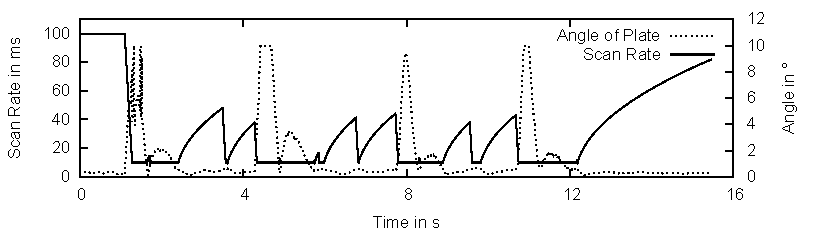
\includegraphics{../figures/selfadapt_a}
	\caption{Scan rate compared to plate's angle}
	\label{fig:selfadapt_a}
\end{figure}
A larger angle of the plate implies that the ball is either far away from the
center or has a high velocity. As figure \ref{fig:selfadapt_a} further
indicates, the increase of the scan rate is performed gradually over time,
while the decrease in case of a disturbance of the ball is done much faster,
more precisely in a linear or exponential fashion, respectively. Furthermore,
it is limited in both its maximal and minimal values. Note, that since the
adaption of the scan rate is performed at a rate equal to the scan rate
itself, the resulting change as seen in the plot is not linear or exponential.

\section{Evaluation}
While the previous sections stated the implementation details of the
demonstrator, this section presents a detailed evaluation regarding relevant
aspects of this work. It addresses the benefits of the newly introduced
techniques like the integration of \ac{HLS} or the hardware interconnect, and
draws conclusions for its feasibility for \acp{PAC}. Furthermore, the
discussed self-adaption strategies are evaluated and to what extend they
influence the system's power consumption.

\subsection{\acl{HLS}}
The ball on plate demonstrator consist out of a variety of hardware threads,
implemented using a combination of Vivado HLS and \ac{VHDL}. During
development it clearly turned out, that \ac{HLS} approaches simplify the
development process and reduce the implementation time significantly.
Especially the advanced debugging capabilities by executing the hardware
implementation in software avoids time consuming \ac{RTL} simulations and
allows to more easily verify the algorithm's correctness. It also clearly
turned out, that \ac{HLS} has its strengths in complex arithmetic calculations
including fixed point data types and divisions, while it is not useful for
implementing timing critical functions. For example, the inverse kinematics
include many fixed point calculations for transformations between the
different coordinate systems, while the implementation of the \ac{SPI}
protocol for the touch controller or the generation of a \ac{PWM} signal for
the servos require clock accurate timing. However, even if a hardware thread
is implemented in either \ac{VHDL} or \ac{HLS}, it can still benefit from
both's advantages by instantiating custom user logic generated using \ac{HLS}
techniques in a \ac{VHDL} thread. For example, the \emph{Touch} thread
instantiates a scaling entity to transform the voltages into coordinates in
the plate's coordinate system. More generally spoken, a thread could be
implemented in \ac{VHDL} and instantiates multiple user logic entities from
different sources, like Vivado HLS or the Core Generator tool.

\subsection{Performance}
Incorporating the \ac{FPGA} into the system and spending spending additional
effort for developing hardware implementations of different threads promises
significant speedups and lower energy consumption. To demonstrate the possible
benefits in utilizing hardware threads, this section presents a performance
evaluation of the system and compares different implementation modes of the
various threads and resources.

Table \ref{tab:demo_perf} and figure \ref{fig:demo_perf} present the measured
performance characteristics, i.e. the execution times, as well as the power
consumptions for different configurations of the system, varying in number and
implementation modes of threads and resources. \emph{HC} and \emph{SC}
indicate the mode of the control thread, \emph{HI} and \emph{SI} the number of
threads solving the inverse kinematics problem and \emph{HIc} and \emph{SIc}
the implementation mode of the resources used for communication between the
different threads.
\begin{table}
	\scriptsize
	\centering
	\captionabove{Performance evaluation of demonstrator}
	\label{tab:demo_perf}
	\begin{tabular}{lccccc}
	\hline
	\textbf{Configuration} & \textbf{Touch (ms)} & \textbf{Control (ms)} & \textbf{Inverse (ms)} & \textbf{Overhead (ms)} & \textbf{Power (W)}\\
	\hline
	HC, 1 HI, HIc & 0.519823 & 0.002807 & 0.988770 & 0.002273 & 3.282711\\
	HC, 2 HI, HIc & 0.518647 & 0.002807 & 0.494335 & 0.002339 & 3.285396\\
	HC, 3 HI, HIc & 0.516636 & 0.002807 & 0.330010 & 0.002188 & 3.285785\\
	%HC, 4 HI, HIc & 0.516841 & 0.002807 & 0.329460 & 0.002298 & 3.282977\\
	HC, 5 HI, HIc & 0.516800 & 0.002807 & 0.329111 & 0.002129 & 3.280403\\
	%HC, 1 SI, HIc & 0.533154 & 0.002807 & 13.985671 & 0.035734 & 3.393689\\
	%HC, 2 SI, HIc & 0.533736 & 0.002807 & 7.096788 & 0.048645 & 3.394321\\
	SC, 1 SI, HIc & 0.533503 & 0.029877 & 14.175555 & 0.085007 & 3.403409\\
	SC, 2 SI, HIc & 0.520863 & 0.028068 & 9.264843 & 0.092866 & 3.393398\\
	SC, 1 HI, SIc & 0.532210 & 0.043583 & 1.236276 & 0.132937 & 3.300271\\
	HC, 1 HI, SIc & 0.516617 & 0.002807 & 1.232297 & 0.154249 & 3.310040\\
	HC, 5 HI, SIc & 0.513496 & 0.002807 & 0.394123 & 0.173940 & 3.305959\\
	\hline
	\end{tabular}
\end{table}
\begin{figure}
	\centering
	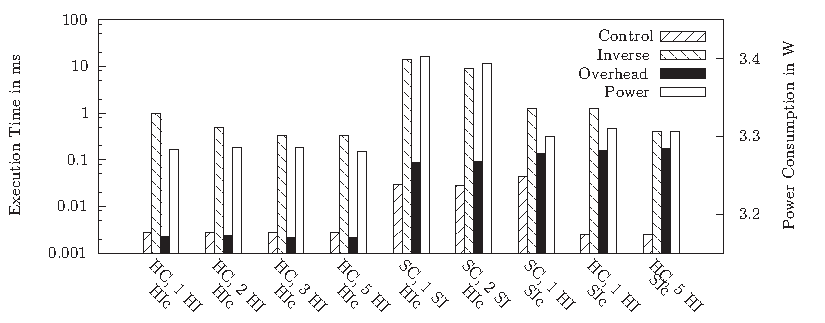
\includegraphics{../figures/demo_perf}
	\caption{Performance evaluation of demonstrator}
	\label{fig:demo_perf}
\end{figure}
The execution times are measured as described in section
\ref{sssec:processing} and listed for the \emph{Touch}, \emph{Control} and
\emph{Inverse} threads. For the \emph{Touch} thread, it does not include the
idle time until the next read, but only the time needed to interface the touch
controller, averaging multiple values and eventually rejecting invalid
measurements. The overhead is calculated by measuring the time needed for the
entire cycle and subtracting the single execution times. Note, that the
execution time of the \emph{Inverse} thread also include communication
overhead, since it represent the time required for calculating all six legs,
determined as the difference of start time of first leg and end time of last
leg. The power is measured utilizing the LTC4151 \ac{IC} as described in
section \ref{sssec:power}. All measurements where averaged over 1000 samples,
acquired during $\SI{20}{\second}$.

As already predicted when designing the system, the inverse kinematics require
the most computation time during the scan cycle and significantly benefits
from a hardware implementation in several aspects. First of all, a single
software thread needs around $\SI{14}{\milli\second}$ for its calculation,
which is far beyond the targeted scan cycle rate of $\SI{10}{\milli\second}$.
Even two software threads are straight at the limit and do not scale linearly,
due to other task executed on the processor. In comparison, the hardware
implementation provides a speedup of 14 with regard to the single thread
configuration and even up to 28 with regard to multiple threads. Furthermore,
the hardware threads scale linearly, i.e. doubling the number of threads
halves the execution time. A single hardware thread takes
$\SI{0.988770}{\milli\second}$, while two hardware threads take
$\SI{0.494335}{\milli\second}$, resulting in a speedup of $\nicefrac{\SI{0.988
770}{\milli\second}}{\SI{0.494335}{\milli\second}}=2.000202$. In applications
requiring even shorter scan cycles, a hardware implementation can provide huge
benefits. Note, that five inverse threads provide no more speedup compared to
three, since in both cases two executions are necessary. Only a sixth thread
would provide a further speedup, but due to resource limitation cause by
insufficent \ac{DSP} blocks, six threads could not be implemented on the
ZedBoard. Not only the processing performance is effected by the
implementation mode, but also the power consumption can be reduced by
incorporating custom hardware. In this case, a difference of around
$\SI{120}{\milli\watt}$ could be measured.

While the \emph{Inverse} thread benefits most considerably from its
acceleration using a custom hardware implementation, the \emph{Control} thread
also achieves a speedup of approximately 10. Since the control algorithm
cannot be parallelized and has significantly lower processing requirements,
this speedup is less prominent and, furthermore, has no influence on the
system's power consumption. However, the hardware implementation offers less
overhead due to the direct communication in hardware and a clearly lower
jitter in execution time. While for this application the jitter is not too
important, it might be relevant for jitter sensitive applications and a reason
for a hardware thread implementation.

Besides the implementation modes of the threads, the modes of the resources
are influencing the performance of the system. As the last rows of table
\ref{tab:demo_perf} indicate, the overhead introduced by the software
resources heavily influences the overall performance. While, for example in
case \emph{HC, 5 HI, HIc} the overhead constitute only 0.64\% of the inverse
and control threads' execution time, in case \emph{HC, 5 HI, SIc}, it account
for 43.82\%. Since it is far below the minimal scan cycle time, the overhead
is still acceptable for this application, but for more low-latency purposes,
it might be an important consideration.

%\subsection{\acl{PAC}}

\subsection{Self-Adaption and Power Consumption}
\begin{figure}
	\centering
	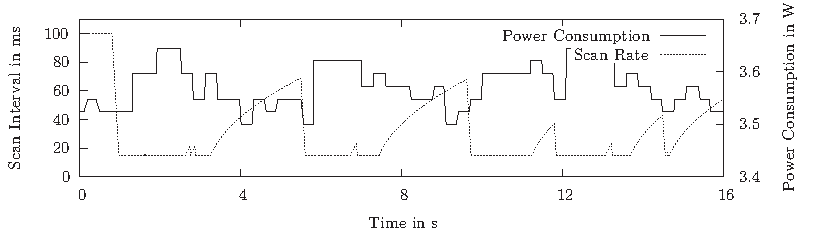
\includegraphics{../figures/selfadapt_pw}
	\caption{Scan rate compared to system's power consumption}
	\label{fig:selfadapt_pw}
\end{figure}
The self-adaption strategy implemented as described in the previous section
tires to minimize the overall power consumption by adapting the cycle rate of
the closed loop controller and, thereby, extending idle periods. Figure
\ref{fig:selfadapt_pw} shows an exemplary execution and how the adaption in
scan rate effects the overall power consumption of the system. It clearly
shows the relation of the two variables and that the system is able to reduce
its power consumption by using self-adaption techniques. However, these
measurements were made with the inverse kinematics calculated in software,
which is, as shown in the previous section, not optimal in terms of processing
performance, but, in general, might be an option if other applications require
resources on the \ac{FPGA}. When investigating the effect of the scan rate
with the inverse kinematics implemented in hardware, no change in power
consumption could be measured via the LTC4151 \ac{IC}. The LTC4151 has a
resolution of $\SI{20}{\micro\volt}$ \citep{LTC4151}, which corresponds to
$\SI{0.024}{\watt}$, and a conversion rate of typically $\SI{7.5}{\hertz}$,
i.e. a single measurement takes around $\SI{130}{\milli\second}$. To get an
impression of the power consumption of the system and verify, that the
expected change is below the measurement accuracy, the already mentioned
XPower tool from Xilinx is used for analysis of the implemented logic. Table
\ref{tab:xpower} shows the power consumption of the threads for different
\ac{FF} toggle rates.
\begin{table}
	\scriptsize
	\centering
	\captionabove{Power consumption estimated by XPower for different \ac{FF}
	toggle rates}
	\label{tab:xpower}
	\begin{tabular}{lccc}
	\hline
	\textbf{Thread} & \multicolumn{3}{c}{\textbf{Power consumption in $\SI{}{\watt}$}}\\
	& \textbf{12.5\%} & \textbf{30\%} & \textbf{100\%}\\
	\hline
	Servo & 0.00023 & 0.00031 & 0.00059\\
	Touch & 0.00557 & 0.00632 & 0.00762\\
	Control & 0.00495 & 0.00530 & 0.00583\\
	Inverse & 0.00622 & 0.00706 & 0.00918\\
	\hline
	& 0.01697 & 0.01899 & 0.02322\\
	\hline
	\end{tabular}
\end{table}
Even with a maximum toggle rate of 100\% the total power consumption of all
processing threads is beneath the resolution of the LTC4151. Furthermore, the
conversion rate is below the slowest possible cycle rate of the system.
Therefore, it is not possible to measure any difference in power consumption.

\subsection{\acs{PID} Controller}
Although the scope of this thesis does not focuses on controller design and
tuning, a brief evaluation of the implemented \ac{PID} controller is given in
this section. By systematically exploring different values for the
\ac{PID} parameters, the final system applies $K_P = -0.09$, $K_I = 0$ and
$K_D = -28$. Figure \ref{fig:demo_pid} shows a tracking of the ball for two
applications.
\begin{figure}
	\centering
	\begin{subfigure}{0.49\textwidth}
		\centering
		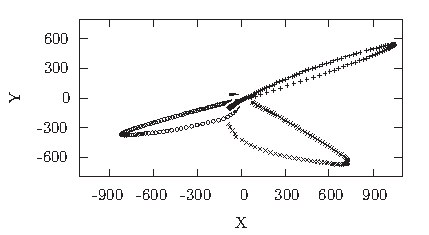
\includegraphics[width=\textwidth]{../figures/eval_pos}
		\caption{Balancing of ball in the center}
		\label{fig:eval_pos}
	\end{subfigure}
	\begin{subfigure}{0.49\textwidth}
		\centering
		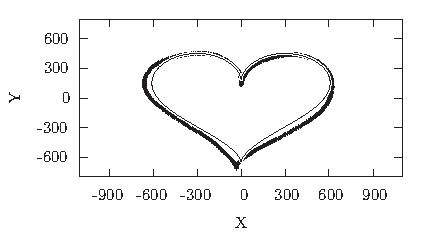
\includegraphics[width=\textwidth]{../figures/eval_traj}
		\caption{Following of a fixed trajectory}
		\label{fig:eval_traj}
	\end{subfigure}
	\caption{Captures of ball's movement controlled by \acs{PID} controller}
	\label{fig:demo_pid}
\end{figure}
For figure \ref{fig:eval_pos} the ball is balanced at the center of the plate
and any external disturbance is compensated, with the aim to keep the ball on
the plate. The figure shows a slight overshoot at the center and, due to a
missing integral term, never reaches the absolute center. Since the ball has a
relatively high initial friction, a large angle is needed to give the ball an
initial impulse. It then destabilizes and never reaches a resting position.
Therefore, a small inaccuracy for its final position is acceptable.
Additionally to the balancing of the ball in the center, figure
\ref{fig:eval_traj} shows an exemplary trajectory for the ball to follow.
Again, an inaccuracy from the desired trajectory in the direction of movement
is apparent. The trajectory is achieved by changing the target position of the
ball over time and adjusting the \ac{PID} controller to avoid the so-called
derivative kick.